\documentclass[a4paper, 12pt, headsepline]{scrartcl}
    % General document formatting
    %\usepackage[margin=0.7in]{geometry}
    %\usepackage[parfill]{parskip}
    \usepackage[utf8]{inputenc}
    %\usepackage[headsepline,footsepline]{scrpage2}
    \usepackage[onehalfspacing]{setspace}
    \usepackage{times}
    \usepackage{graphicx}
    \graphicspath{ {images/} }


% Header and Footer Formatting-----------------------------------------------------------------------
%   Formatting of Header and Footer
% ---------------------------------------------------------------------------------------------------
%\pagestyle{scrheadings}
%\clearscrheadfoot
%\ohead{\headmark}
%\ofoot{\pagemark}

% TODO: make itemize neater

% Center all images
\makeatletter
\g@addto@macro\@floatboxreset\centering
\makeatother

% Title Page Information-----------------------------------------------------------------------------
%   These are the informations printed on the title page of the article
% ---------------------------------------------------------------------------------------------------

\title{Project trckr}
\subtitle{Technical Article}
\date{May 2018}
% TODO: authors more compact? 
\author{
Ankeshian, Gabriel\\
\texttt{ankesgab@students.zhaw.ch}
\and
Balidis, Dimitri\\
\texttt{baliddim@students.zhaw.ch}
\and
Christen, Luca\\
\texttt{chrisluc@students.zhaw.ch}
\and
Jossi, Savino\\
\texttt{jossisav@students.zhaw.ch}
\and
Milenkovic, Daniel\\
\texttt{milendan@students.zhaw.ch}
\and
Nominato, Angelica Helena Moreira Alves\\
\texttt{moreiane@students.zhaw.ch}
\and
Pacassi, David\\
\texttt{pacasdav@students.zhaw.ch}}

\begin{document}
\maketitle
\pagebreak

% Proofreading Checklist
% * avoid passive voice
% * succinct sentences
% * use active voice
% * did I say don't use passive voice?

% Abstract----------------------------------------------------------------------
%   This is the abstract of the technical article
% ------------------------------------------------------------------------------
\begin{abstract}
  The main goal of the present article is to describe the idea, goals and main
  functionalities of the web based application trckr. We developed trckr for
  % Since we want trckr to be all lowercase, we avoid using it at the start of
  % the sentence
  everyone who works on a project and needs an intuitive and simple web tool to
  accurately track their time spent on different tasks.
  % Hint: Empty line makes a paragraph which is semantically different from the
  % forced \\ newline (and much neater)

  The backend is written in Python with the help of the web application
  framework Django and the frontend with the Javascript UI framework Vue.js.
  Both technologies were new to most team members, but have proven themselves
  effective and learning them were ultimately a benefit the outcome of the
  project.

  In order to compete with similar tools and web services, trckr focuses on
  performance and usability. To distinguish trckr from the competition, many
  features are planned to manage projects and tasks in a user-friendly manner.
  This will allow the user to leverage trckr to handle the ever increasing
  complexity in project management and task tracking found in large companies.
  Despite being targeted at large companies, trckr will remain open source and
  anybody can contribute, covering cases we might have never dreamed of.
\end{abstract}

\clearpage

% Table of Contents-------------------------------------------------------------
%   This is the table of contents
% ------------------------------------------------------------------------------

\tableofcontents

\clearpage

% Introduction------------------------------------------------------------------
%   This is the information printed on the title page of the article
% ------------------------------------------------------------------------------
\section{Introduction}
Time and task tracking are important activities in many businesses to gain
insights on the productivity of a team, requiring appropriate tools allowing
easier and more accurate time tracking. Many processes and methods have been
developed in the past to cover this need. Unfortunately most of them address
just a certain need or have been fine tuned to a specific company or team. This
necessarily leads to a loss of experience that could have been leveraged by
other teams but is also not generic enough to adapt to different processes,
causing other companies to inappropriately adapt to the tool instead of the tool
adapting to the company.

\subsection{Objectives}
The goal with trckr is to develop and distribute a time tracking web application
that is easy to understand and use. The most important requirement is to
require just a few steps to track all the required information. Only this will
keep the user engaged and raise the accuracy of the provided data.

\subsection{Main Features}
The user is able to:
\begin{itemize}
    \item register and login to trckr
    \item create and edit projects
    \item create, track and edit tasks
    \item visit trckr on any device
\end{itemize}

\section{Technologies}
\subsection{Django}
Django is an open source web framework written in Python. It encourages fast,
clean and simple development of web applications. One of the main advantages is
it's fast setup, enabling the developer to create applications swiftly through
it's Model-View-Presenter scheme. Django also comes with support for various
databases. Many users compare Django to Ruby On Rails but written in Python.
Django also follows the DRY principle (Don't Repeat Yourself).

\subsection{PostgreSQL}
A PostgreSQL database stores all the data for trckr. PostgreSQL is fully
supported by Django and configuration and management is minimal, because the
database access is handled by Django.

\subsection{Vue.js}
Vue.js is a progressive framework for building user interfaces.\cite{vuejs}
Vue.js is used for trckr mainly for its simplicity and the rather shallow
learning curve it provides to unexperienced developers. The features that Vue.js
provides allow the creation of data structures that can easily be displayed in
on a website. This and the ability to easily make calls to the backend make it a
good fit for trckr.


% Results-----------------------------------------------------------------------
%   This is the information printed on the title page of the article
% ------------------------------------------------------------------------------
\section{Results}
The architecture was kept fairly simple, as illustrated in figure
\ref{fig:architecture}, using Django with PostgreSQL in the backend and a
frontend based around Vue.js.

\begin{figure}[h]
    \includegraphics[width=8cm]{architecture}
    \caption{Architecture of trckr}
    \label{fig:architecture}
\end{figure}

\subsection{API}
The backend of the trckr application implements a RESTful API using the Django
REST framework. The API provides basic CRUD operations for all the entities
available in the database. There are five main endpoints to retrieve and save
data on the server: authentication, user, projects, tasks and time entries. Except
for the authentication and user endpoints, all endpoints need an authentication
token to be accessed.

\subsubsection{Endpoints}
\begin{description}
\item[authentication] allows users to retrieve an authentication token from the
  server to access the other parts of the API. Via this endpoint, one can also
  invalidate the token.
\item[user] is only used to create new user accounts.
\item[projects] lets user create, read, update and delete projects as well as
  display all the tasks associated with a project.
\item[task] used to create, read and update tasks for a given project. There
  also exits a way to list all relevant time entries for a task.
\item[time entries] also used for create, read, update and delete operations
\end{description}

Each object of an entity has a unique ID. This ID can be used to retrieve
information for that specific object by providing it in the URL when calling the
server. This is necessary when updating an object via a POST request.

\subsection{User Interface}

\begin{figure}[h]
    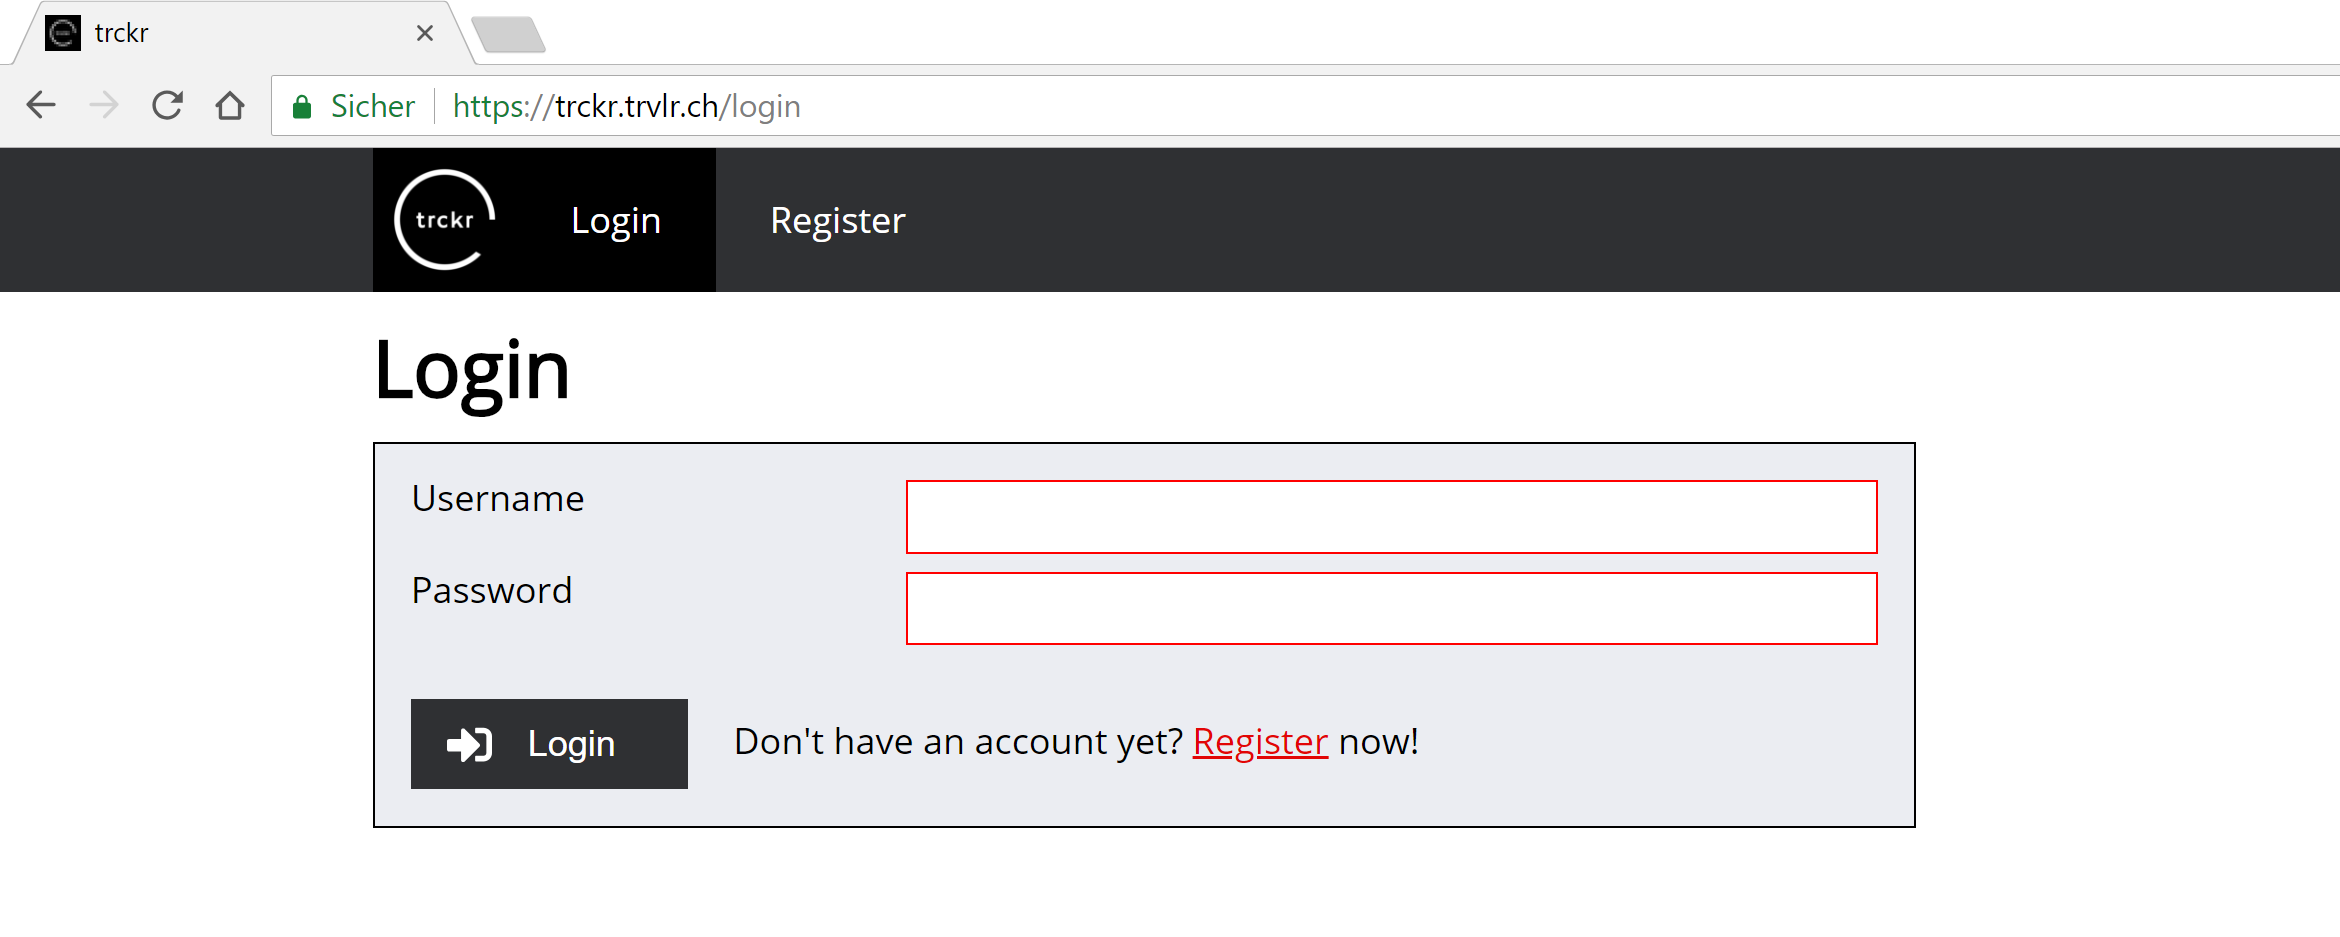
\includegraphics[width=0.8\textwidth]{trckr-login}
    \caption{The trckr login page.}
    \label{fig:trckr-login}
\end{figure}

\begin{figure}[h]
    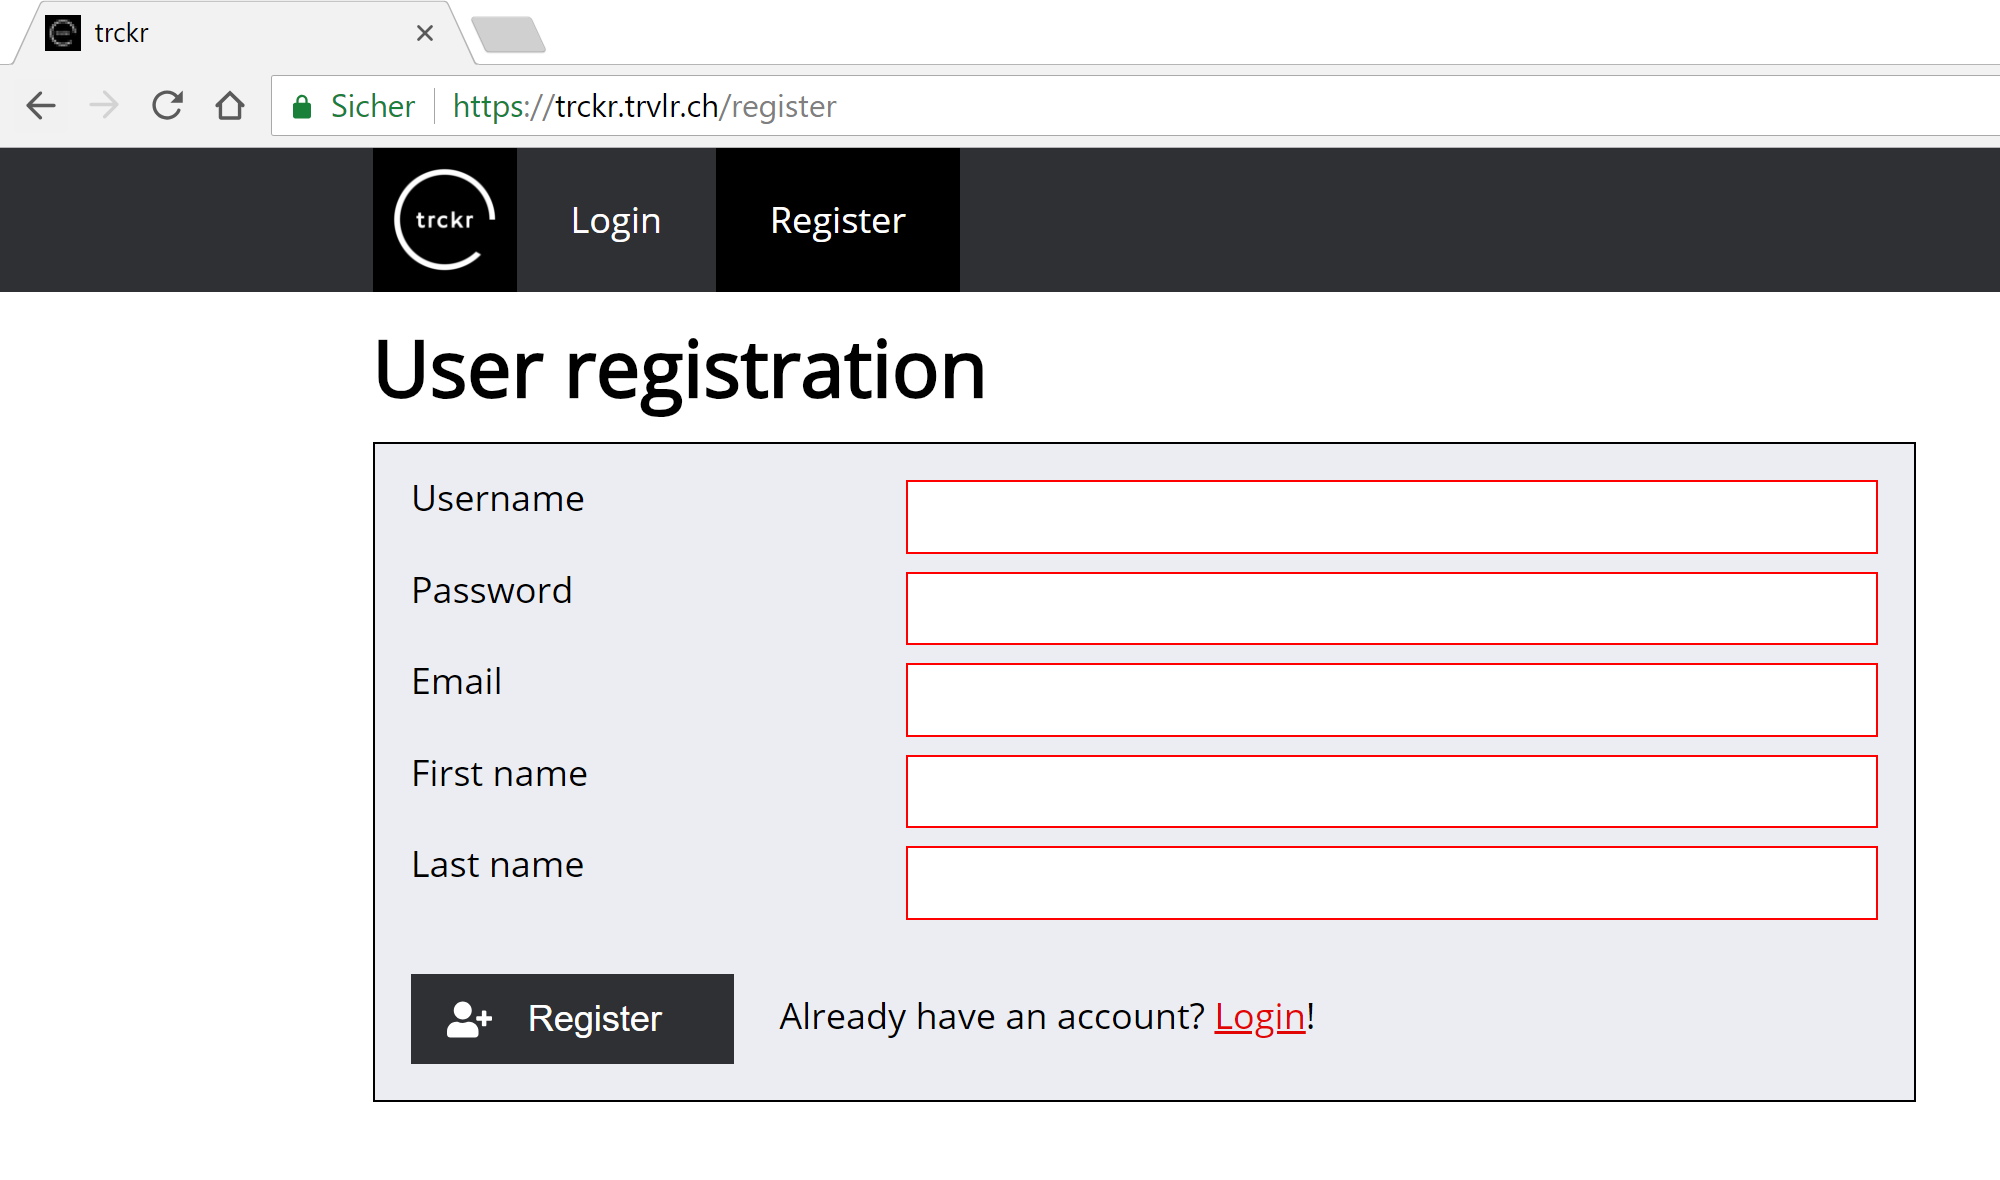
\includegraphics[width=0.8\textwidth]{trckr-register}
    \caption{The trckr registration page.}
    \label{fig:trckr-register}
\end{figure}

The first thing one sees when visiting trckr, is that there is a login page.
For people that are not yet registered there is the option to register through a
"Register" link. Filling out the registration form will trigger a call to the
backend to create a user. The response to this call will contain an authentication
token, this allows the user to be logged in directly after registering.
Similarly, when submitting the login form the backend will reply with an
authentication token that allows an existing user to be logged in.\\
At the moment of registration the navigation bar on the top of the interface
will contain a link to the dashboard, the projects page, the time entries page
as well as a logout button.\\
The dashboard displays graphs...TODO \\

\begin{figure}[h]
    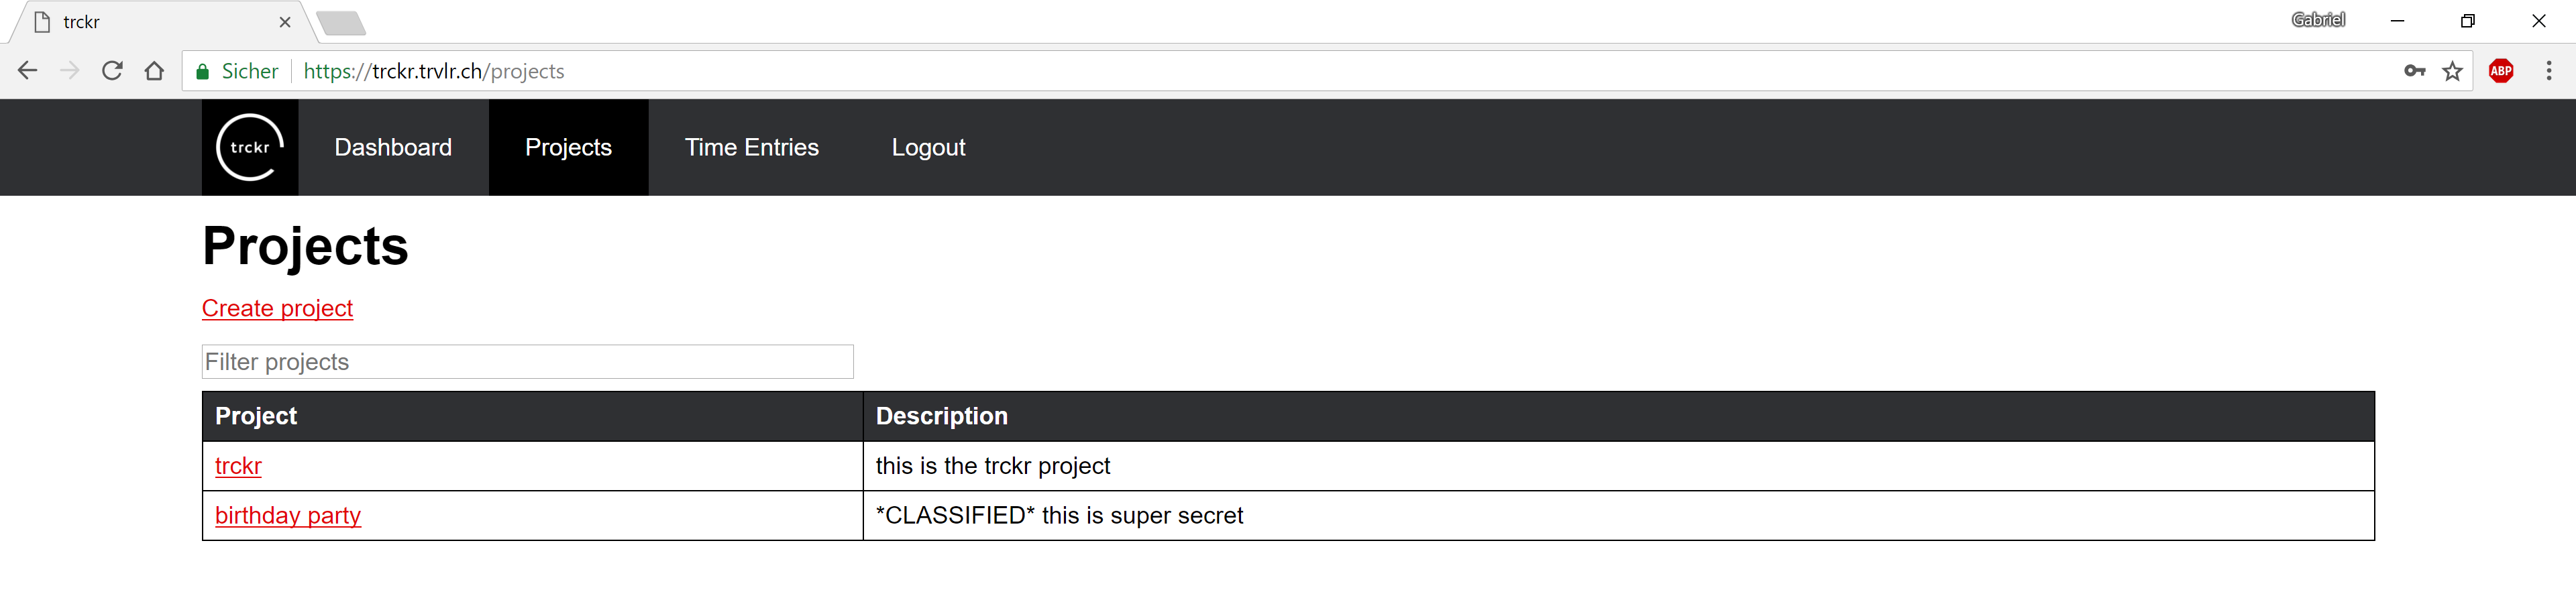
\includegraphics[width=\textwidth]{trckr-projects-table}
    \caption{The projects page.}
    \label{fig:trckr-projects-table}
\end{figure}

On the projects page one can see a table of all the projects that the currently
logged in user is a part of. The table is automatically generated by Vue.js and
it contains a row for each project. Above the projects table there is a
textfield that allows a user to filter for a project or a group of projects that
contain the given substring. To create a new project a user will have to
navigate to the projects page and click on the "Create project" link which will
open the project creation form. In this form a user can specify a name for the
project as well as an optional description.\\
Each project can be viewed in more detail when the project inside the table is
clicked. As the figure below is showing, the project page will contain the name,
the description and a table of all the tasks in the current project.

\begin{figure}[h]
    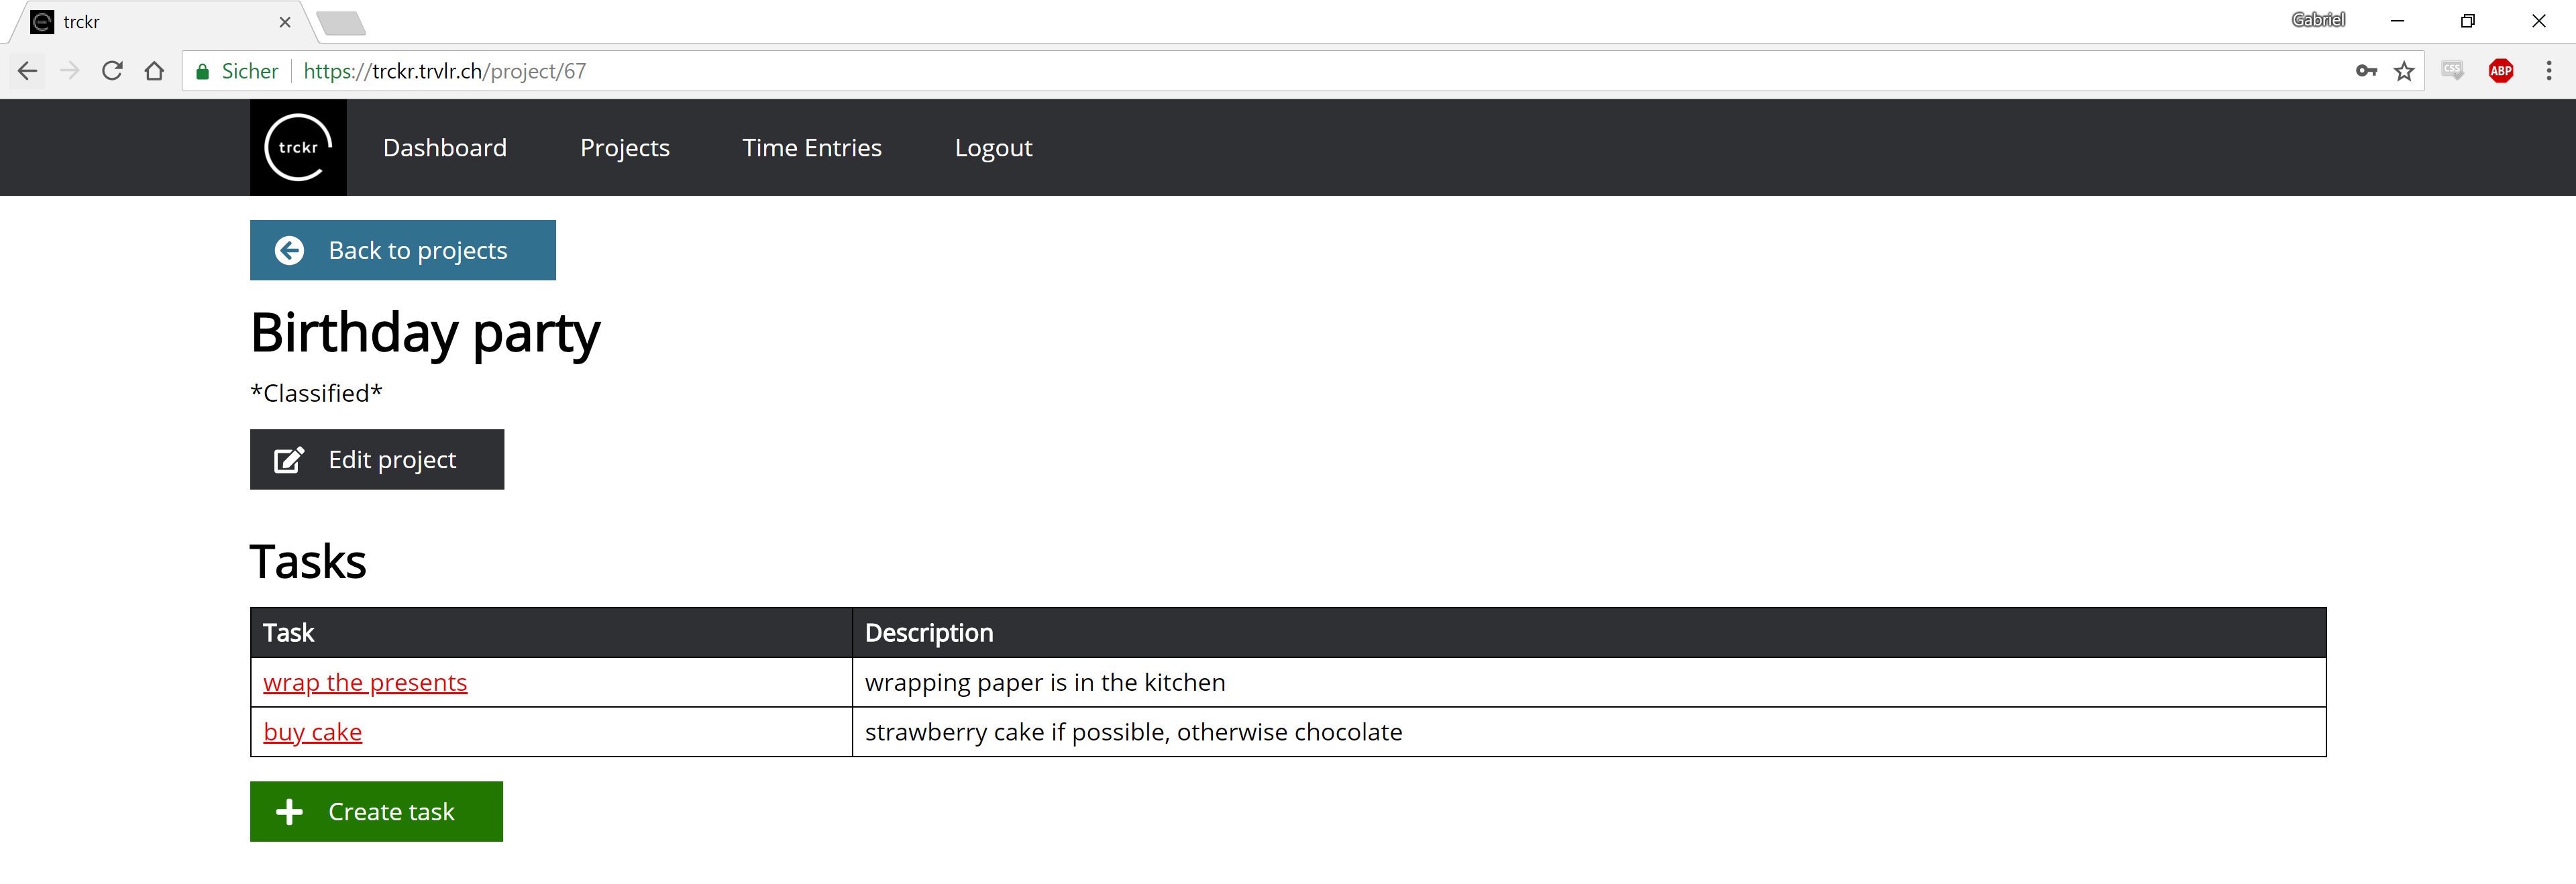
\includegraphics[width=\textwidth]{trckr-project-page}
    \caption{The projects page with the table of all projects.}
    \label{fig:trckr-project-page}
\end{figure}

Clicking on a task will display the details of said task, at the current state
that is only the name and the description of the task.\\
On the "Time Entries" page a user can create a time entry for a specific task of
a project. There is a link on the page that leads to the time entry form. In
said form the user has to choose a project first and then a task of the project
for which the time entry should be created.

\begin{figure}[h]
    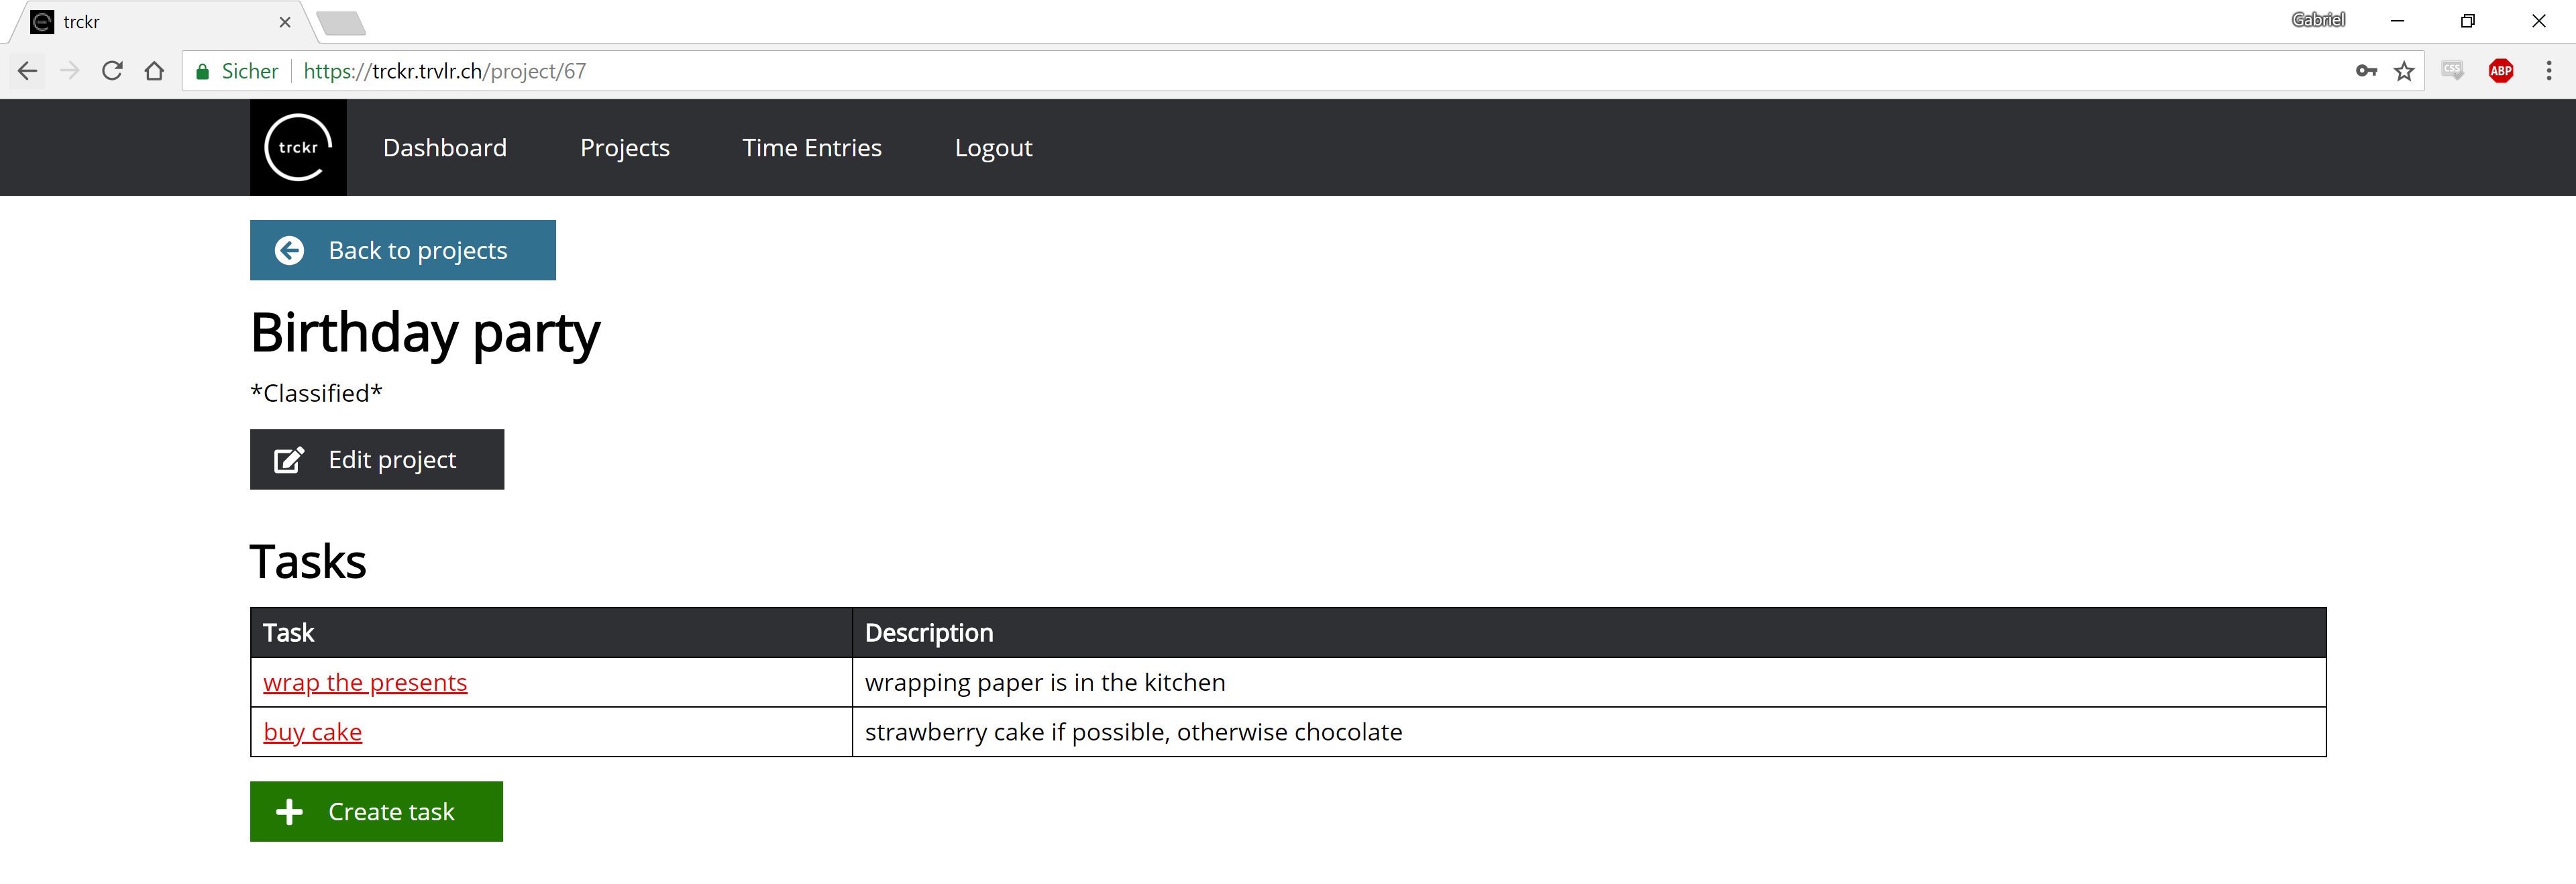
\includegraphics[width=\textwidth]{trckr-project-page}
    \caption{The form to add a time entry to a task.}
    \label{fig:trckr-create-time-entry}
\end{figure}

All time entries will be displayed on the time entry page.

% Outlook----------------------------------------------------------------------------
%   These are the informations printed on the title page of the article
% -------------------------------------------------------------------------------------------
\section{Outlook}
Outlook...

% Conclusion-----------------------------------------------------------------------------
%   These are the informations printed on the title page of the article
% -------------------------------------------------------------------------------------------
\section{Conclusion}
Conclusion...

% Bibliography-----------------------------------------------------------------------------
%   These are the informations printed on the title page of the article
% -------------------------------------------------------------------------------------------
\section{Bibliography}
Bibliography...
\begin{thebibliography}{9}

    \bibitem{vuejs}
    https://vuejs.org/ ; as 10.05.2018


\end{thebibliography}

\listoffigures

\end{document}
